\documentclass[11pt,a4paper]{article}
\usepackage[top=3cm, bottom=2cm, left=2cm, right=2cm]{geometry}
\usepackage[utf8]{inputenc}
% \usepackage[T1]{fontenc}
\usepackage{amsmath, amsfonts, amssymb}
\usepackage{siunitx}
\usepackage[brazil]{babel}
\usepackage{graphicx}
\usepackage[margin=10pt,font={small, it},labelfont=bf, textfont=it]{caption}
\usepackage[dvipsnames, svgnames]{xcolor}
\DeclareCaptionFont{MediumOrchid}{\color[svgnames]{MediumOrchid}}
\usepackage[pdftex]{hyperref}
\usepackage{natbib}
\bibliographystyle{plainnat}
\bibpunct{[}{]}{,}{s}{}{}
\usepackage{color}
\usepackage{footnote}
\usepackage{setspace}
\usepackage{booktabs}
\usepackage{multirow}
\usepackage{subfigure}
\usepackage{fancyhdr}
\usepackage{leading}
\usepackage{indentfirst}
\usepackage{wrapfig}
\usepackage{mdframed}
\usepackage{etoolbox}
\usepackage[version=4]{mhchem}
\usepackage{enumitem}
\usepackage{caption}
\usepackage{titlesec}
\usepackage{tcolorbox}
\usepackage{tikz}
\usepackage{LobsterTwo}
\usepackage[T1]{fontenc}
\usepackage{fontspec}
\usepackage{txfonts}
\AtBeginEnvironment{equation}{\fontsize{13}{16}\selectfont}


\titleformat{\section}{\LobsterTwo\LARGE\color{CarnationPink}}{\thesection.}{1em}{}
\titleformat{\subsection}{\LobsterTwo\LARGE\color{CarnationPink}}{\thesubsection}{1em}{}


\DeclareCaptionLabelFormat{figuras}{\textcolor{DarkTurquoise}{Figura \arabic{figure}}}
\captionsetup[figure]{labelformat=figuras}

\makeatletter
\renewcommand\tagform@[1]{\maketag@@@{\color{CarnationPink}(#1)}}
\makeatother

\renewcommand{\theequation}{Eq. \arabic{equation}}
\renewcommand{\thefigure}{Fig. \arabic{figure}}
\renewcommand{\thesection}{\textcolor{CarnationPink}{\arabic{section}}}

\setlist[itemize]{label=\textcolor{CarnationPink}{$\mathbf{\square}$}}

\setlist[enumerate]{label=\textcolor{CarnationPink}{\arabic*.}, align=left}


\newcounter{exemplo}

\NewDocumentEnvironment{exemplo}{ O{} }{%
\allowbreak
\setlength{\parindent}{0pt}
  \begin{mdframed}[
  leftline=true,
  topline=false,
  rightline=false,
  bottomline=false,
  linewidth=2pt,
  linecolor=CarnationPink,
  frametitlerule=false,
  frametitlefont=\LobsterTwo\large\color{CarnationPink},
  frametitle={\color{CarnationPink}\LobsterTwo\large #1},
  ]
}{%
  \end{mdframed}
}

\setlength{\fboxsep}{5pt}
\setlength{\fboxrule}{1.5pt}
\usepackage{float}
\renewcommand{\thefootnote}{\alph{footnote}}
\usepackage{url}
\hypersetup{
	colorlinks=true,
	linkcolor=DarkTurquoise,
	filecolor=DarkTurquoise,      
	urlcolor=DarkTurquoise,
	citecolor=DarkTurquoise,
	pdftitle={Radioterapia}
}
\pagestyle{fancy}
\fancyhf{}
\renewcommand{\headrulewidth}{0pt}
\rfoot{Página \thepage}

\title{\LobsterTwo\Huge{Radiobiologia}}
\author{\LobsterTwo{Carcinogênese\nocite{*}}}
\date{\LobsterTwo\textit{Dalila Mendonça}}
\begin{document}
	\maketitle


\section{Introdução}

    O câncer resulta de um acúmulo de múltiplas mutações em genes celulares que regulam o crescimento celular/tempo de vida, morte e migração, resposta imune, comprimento dos telômeros, instabilidade genômica, invasão e metástase. Algumas mutações são herdadas, enquanto a maioria das outras são espontâneas ou induzidas. As mutações podem aumentar a atividade dos oncogenes ou diminuir a atividade dos supressores tumorais. As várias etapas na evolução de uma célula normal para uma célula cancerosa podem ser classificadas como iniciação, promoção e progressão. As células cancerígenas devem desenvolver a capacidade de se dividir descontroladamente, mantendo o comprimento dos telômeros, recrutar vasculatura através do VEGF e alterar a adesão célula-célula para invadir e metastizar. Uma melhor compreensão da genética do tumor levou à terapia direcionada contra o câncer, com anticorpos monoclonais e inibidores de pequenas moléculas direcionados a moléculas específicas e vias moleculares desreguladas em cânceres humanos.

\section{Mudanças Genéticas no Câncer}

    A análise das células cancerígenas mostra que a maioria delas tem DNA altamente anormal, com múltiplas alterações em comparação com as células saudáveis. 
    
    Podem ocorrer diferentes tipos de mutações em uma célula e que são ocasionadas por diferentes mecanismos. Algumas mutações são de origem hereditárias, e estão presentes desde o nascimento. Por exemplo, as mutações BRCA1/2 causam câncer de mama/ovário hereditário; As mutações FAP e MSH/MLH causam câncer de cólon hereditário; Mutações Rb causam retinoblastoma hereditário e sarcomas de partes moles; As mutações da p53 causam a síndrome de Li-Fraumeni, com múltiplas malignidades.
    
    Outras mutações ocorrem de forma espontânea onde as mutações ocorrem aleatoriamente devido ao envelhecimento da célula, oxidação e devido aos processos de replicação e de mitose do DNA. A maiorias das mutações que conduzem à carcinogênese são de caráter espontâneo, provavelmente devido à instabilidade genômica, onde a perda de reparo do DNA, perda processos de morte celular como apoptose e perda de vias de senescência levam ao acúmulo de mutações espontâneas ao longo do tempo.

    Mutações quimicamente induzidas devido a agentes químicos, como o tabaco, causam, preferencialmente, mutações pontuais devido à danos às bases ou reticulação do DNA (crosslinking). Ja as mutações radio-induzidas tendem a ser mutações grosseiras (cromossômicas), pois causam quebras duplas no DNA.

    Algumas anormalidades nos genes são causadas por vírus, como o HPV que é o vírus amplamente divulgado responsável pelo câncer de colo de útero e alguns cânceres de cabeça e pescoço e o EBV que está associado a diferentes tipos de câncer em diferentes regiões do mundo. 
    
    \begin{itemize}[label=\textcolor{CarnationPink}{$\blacktriangleright$}]
        \item A proteína E6 do vírus do papiloma humano (HPV E6) tem a capacidade de se ligar à proteína supressora de tumores p53, que é responsável por controlar o crescimento celular e induzir a morte celular programada (apoptose) quando necessário; No entanto, a proteína HPV E6 direciona a proteína p53 para ser degradada, ou seja, ela impede que a proteína p53 cumpra sua função normal de controle do ciclo celular e da morte celular o que leva a uma desregulação do ciclo celular e à inibição dos processos de morte celular, como a apoptose, que são mecanismos importantes para eliminar células danificadas ou com potencial de se tornarem cancerosas.
        \item Já a proteína E7 do vírus do papiloma humano (HPV E7) em a capacidade de se ligar à proteína do retinoblastoma (Rb), que é responsável por controlar a progressão do ciclo celular. Ao direcionar a proteína Rb, a HPV E7 perturba a regulação normal do ciclo celular. Isso significa que o ciclo celular, que normalmente segue uma sequência de eventos bem coordenada e controlada, é interrompido e desregulado que pode levar a um crescimento celular descontrolado e ao acúmulo de células anormais, característico de malignidades.
        \item o Vírus Epstein-Barr (EBV) também chamado de herpesvírus humano 4, é responsável por causar a mononucleose, uma doença caracterizada por febre, dor de garganta, fadiga e aumento dos linfonodos. Além disso, na China e no Sudeste Asiático, o EBV é responsável por alguns cânceres de nasofaringe, que afetam a região da garganta atrás do nariz. Na África, o EBV está associado ao linfoma de Burkitt, um tipo de câncer que afeta os linfonodos. As proteínas de membrana latente do VEB (LMP1 e LMP) e os antígenos nucleares do EBV têm a capacidade de interferir na sinalização celular, especialmente nos processos de proliferação celular, metástase (disseminação do câncer para outras partes do corpo) e morte celular programada (apoptose). Essa interrupção da sinalização celular pode contribuir para o desenvolvimento e progressão dos cânceres associados ao EBV.
    \end{itemize}

    Quanto às mudanças epigenéticas (aquelas que alteram a função genética), a mais comum para o câncer são a metilação e a acetilação. Essas mudanças estão associadas à mudanças na cromatina onde a metilação diminui a expressão genética enquanto que a acetilação aumenta a expressão genética.
    
    O silenciamento epigenético é causado principalmente por promotores de hiper-metilação do gene. Nestes casos, a célula cancerígena utiliza o mecanismo de metilação para degradar os genes de supressão tumoral e de reparo do DNA e isso pode deixá-los vulneráveis à agentes externos que danificam o DNA como quimioterápicos e Radioterapia. Por exemplo, a metilação de MGMT no glioblastoma se correlaciona com a resposta à temozolomida (quimio).

\section{Tipos de Tumores}

    Os tumores podem ser classificados como benignos, pré-malignos e tumores malignos. Essas classificações são baseadas baseadas em suas características e comportamento biológico e normalmente são definidas a partir de um exame histopatológico que avalia as características microscópicas das células.

    Um \textcolor{CarnationPink}{tumor benigno} se tata de células não cancerígenas, onde as células do tumor se assemelham às células normais e têm estrutura e função semelhantes. Geralmente estas células crescem de forma lenta e localizada e tendem a ser circunscritos e bem delimitados, sem invadir tecidos adjacentes.Portanto, essas células raramente se espalham para outras partes do corpo causando metástases. Geralmente os tumores benignos não causam problemas graves, a menos que cresçam em locais críticos que interfiram com funções vitais.

    \begin{wrapfigure}{r}{0.5\textwidth}
        \centering
        \fcolorbox{DarkTurquoise}{white}{%
            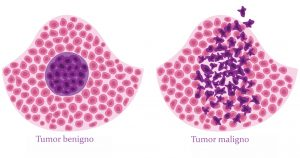
\includegraphics[width=0.48\textwidth]{Imagens/tumorbenignoEMaligno.jpg}
        }%
    \end{wrapfigure}

    Os \textcolor{CarnationPink}{tumores pré-malignos} também conhecidos como lesões pré-cancerígenas ou lesões displásicas. Essas lesões têm alterações celulares anormais que as distinguem das células normais, mas ainda não são consideradas cancerígenas. Os tumores pré-malignos podem ser um estágio intermediário entre o tecido normal e o câncer e têm maior potencial de progredir para um tumor maligno ao longo do tempo. A identificação precoce e o tratamento de lesões pré-malignas podem ajudar a prevenir o desenvolvimento de câncer.

    Os \textcolor{CarnationPink}{tumores malignos} são tumores cancerígenos. As células do tumor sofrem alterações genéticas e epigenéticas que afetam sua estrutura e função normais e crescem de forma descontrolada e invasiva, infiltrando-se em tecidos circundantes. Os tumores malignos podem se espalhar para outras partes do corpo por meio da metástase, formando tumores secundários em locais distantes e podem interferir nas funções normais do corpo causando sintomas graves. 


\section{Modelo de Progressão Tumoral}

    O câncer é uma doença de proliferação descontrolada, invasão, metástase, angiogênese e evitação imunológica. Geralmente são necessárias muitas mudanças para transformar uma célula normal em uma célula cancerosa. 

    O modelo de vários passos da carcinogênese, também conhecido como modelo de progressão tumoral, é uma teoria proposta para descrever o processo pelo qual o câncer se desenvolve ao longo do tempo. Esse modelo sugere que o desenvolvimento do câncer ocorre em estágios sequenciais, onde o câncer se desenvolve a partir de uma célula normal em um processo gradual e acumulativo, de modo que  cada etapa é caracterizada por alterações genéticas e epigenéticas adicionais que conferem vantagens seletivas às células cancerígena. A \ref{fig:carcinogeneseMultiPassos} mostra o modelo de vários passos da carcinogênese onde múltiplas mutações são necessárias para que uma célula normal se transforme em célula cancerosa, e para isso a célula passa pelas etapas de iniciação, promoção e progressão até o desenvolvimento de metástases.  

    \begin{figure}[h]
        \centering
        \fcolorbox{DarkTurquoise}{white}{%
            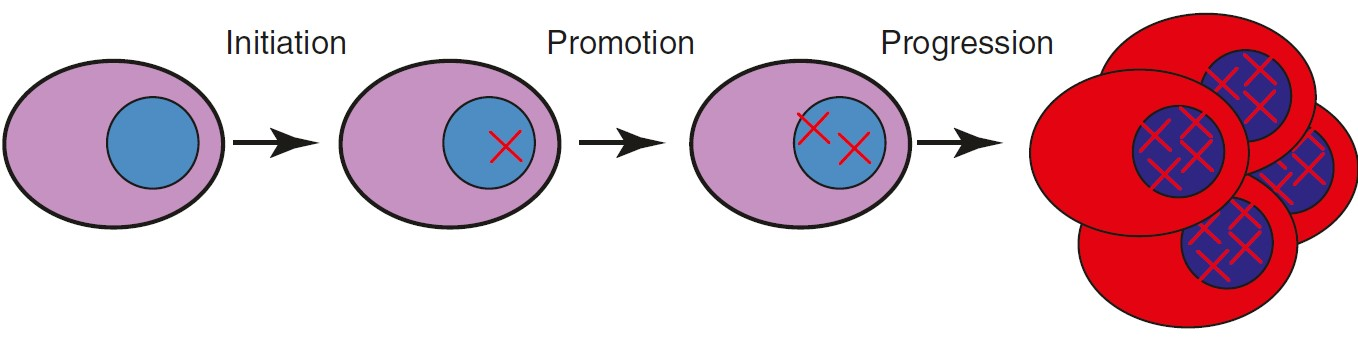
\includegraphics[width=0.8\textwidth]{Imagens/carcinogeneseMultiPassos.jpg}
        }%
        \caption{Modelo de Progressão Tumoral}
        \label{fig:carcinogeneseMultiPassos}
    \end{figure}

    \begin{enumerate}
        \item \textcolor{DarkTurquoise}{\textbf{Iniciação:}} Nesta fase, uma mutação ou dano genético ocorre em uma célula normal. Isso pode ser causado por fatores ambientais, como produtos químicos carcinogênicos, radiação ou vírus. A mutação inicial geralmente afeta genes supressores de tumor ou genes reguladores do ciclo celular.
        \item \textcolor{DarkTurquoise}{\textbf{Promoção:}} Nesta etapa, as células iniciadas são expostas a estímulos que promovem seu crescimento descontrolado. Esses estímulos podem ser agentes químicos, hormônios, inflamação crônica ou outros fatores que estimulam a proliferação celular.
        \item \textcolor{DarkTurquoise}{\textbf{Progressão:}} Nessa fase, ocorrem mutações e alterações genéticas adicionais que levam à formação de um tumor maligno. As células cancerígenas adquirem características invasivas e têm maior potencial de disseminação para outras partes do corpo.
        \item \textcolor{DarkTurquoise}{\textbf{Metástase:}} A metástase ocorre quando as células cancerígenas se separam do tumor primário e se espalham para outras partes do corpo, formando tumores secundários em locais distantes. Isso ocorre quando as células adquirem a capacidade de invadir os tecidos circundantes e entrar na corrente sanguínea ou no sistema linfático.
    \end{enumerate}

    Analises genéticas de doenças do cólon mostram que as mutações que levam a tumores benignos, pré-malignos e malignos ocorrem em etapas específicas do modelo de progressão. As mutações que conduzem à tumores benignos ocorrem normalmente na iniciação, como ocorre com o adenoma de cólon. As mutações que levam à tumores pré malignos são mais comuns na promoção, que é o caso do adenoma displásico dd cólon. Já os tumores malignos são enunciados majoritariamente devido à mutações na progressão, como ocorre no câncer invasivo de cólon. 


\section{Aplicações Clínicas Baseadas na Genética Tumoral}

    As técnicas de perfil genético permitem uma análise da expressão genética tumoral o que favorece nas decisões prognósticas e terapêuticas. Com base nas medidas das expressões genéticas é possível prever o comportamento do tumor e a resposta ao tratamento, através de painéis de prognóstico genéticos, afim de determinar a viabilidade de aplicação de terapias citológicas e terapias direcionadas.

    A \textbf{\textcolor{CarnationPink}{terapia citológica (quimioterapia clássica)}} danifica o DNA ou inibe as vias metabólicas comuns a muitas células humanas. Neste caso a genômica é utilizada para prever a eficácia de drogas citológicas (quimioterápicos) além de prever a possível toxicidade destas drogas.
    
    A \textbf{\textcolor{CarnationPink}{terapia direcionada}} tem como objetivo inibir vias de sinalização celular específicas. Na terapia direcionada, a genômica é utilizada para identificar vias ou mutações celulares específicas que podem ser alvo de drogas. 

\section{Oncogene e Supressores de Tumor}

    Um oncogene é um gene que tem o potencial de causar câncer quando sofre mutações ou é ativado de maneira anormal. De modo geral, um oncogene é um gene que estimula a formação de um tumor através da estimulação da proliferação, estimulação da sobrevivência (anti-apoptose) e através da inibição de supressores de tumor. 

    Os supressores de tumor, ao contrário dos oncogenes, são genes que inibem ou previnem a formação tumoral. Os supressores de tumor podem promover a parada do ciclo celular, promover a apoptose, promover o reparo do DNA e inibir os oncogenes. Os genes Rb e p53 são supressores de tumor que causam a parada do ciclo celular na fase G1, além disso o gene p53 também causa a parada na fase G2. Tanto o Rb quanto a p53 são pró apoptose. O gene NF1 (neurofibromatose tipo 1) age através da inibição do oncogene Ras. Os genes BRCA1/2 e MLH/MSH atuam no reparo do DNA e tem grande predisposição para desenvolvimento cancerígeno caso sofram mutação ou sejam danificados.

    O oncogene surge a partir da mutação, amplificação ou superexpressão de um proto-oncogene, que é a versão do oncogene em normal funcionamento. Já os supressores de tumor podem ser desativados através de mutações ou silenciamento epigenético.

\section{Sinalização Oncogênica e Radioterapia}

    A proteína p53 tem grande envolvimento na resposta ao Dano do DNA e é percebida sua mutação em aproximadamente 50\% dos tipos de câncer que ocorrem em humanos.

    As células deficientes em p53 são deficientes em reparo do DNA radio-induzido, parada do ciclo celular e apoptose. Isso pode levar a uma maior radiossensibilidade devido a perda da capacidade de reparo e parada do ciclo celular. 

    O gene NF-$\kappa$B é uma molécula sinalizadora pró-inflamatória e pró-sobrevivência que está comumente super-expressa em células cancerígenas. Células tumorais com níveis normais de NF-$\kappa$B tendem a sofrer apoptose como resposta a radiação. Já as células com altos níveis de NF-$\kappa$B tendem a ser altamente resistentes à apoptose induzida pela radiação. 

\section{Senescência}

    Uma célula que normalmente é capaz de se multiplicar pode parar de se dividir por vários motivos: sinalização extrínseca, perda de nutrientes, danos ao DNA e assim por diante.

    A senescência é um estado celular irreversível caracterizado por uma parada permanente do ciclo celular e perda da capacidade proliferativa. É um mecanismo de supressão do crescimento celular que ocorre como resposta a vários estímulos, como dano ao DNA, estresse celular, ativação de oncogenes ou envelhecimento normal. Portanto,durante a senescência, as células permanecem metabolicamente ativas, mas não se dividem mais. As células senescentes exibem um aumento na atividade da enzima beta-galactosidase, que é detectável pelo teste de coloração de beta-galactosidase.

    A senescência é considerada um mecanismo de proteção contra o câncer, uma vez que inibe o crescimento descontrolado das células danificadas ou potencialmente cancerígenas. No entanto, à medida que o envelhecimento avança, um acúmulo progressivo de células senescentes pode contribuir para o envelhecimento e para o desenvolvimento de doenças relacionadas à idade.

\section{Telômeros e o Câncer}

    Nas células eucarióticas, o DNA é organizado em cromossomos lineares dentro do núcleo celular diferentemente das bactérias, que possuem DNA circular. Alguns problemas devido a linearidade do DNA são:

    \begin{itemize}
        \item \textcolor{DarkTurquoise}{\textbf{Extremidades adesivas (pegajosas):}} permitem que ocorra uma união indesejada entre extremidades que podem levar a mutações genéticas e a formação de pontes de anáfase\footnote{As pontes de anáfase são estruturas anormais observadas durante a fase de anáfase da divisão celular, indicando problemas na segregação correta dos cromossomos. São visíveis como estruturas finas que conectam os cromossomos nos polos opostos da célula durante a separação.}.
        \item \textcolor{DarkTurquoise}{\textbf{Não pode ser completamente replicado:}} durante a replicação do DNA linear, ocorre uma pequena perda de material genético nas extremidades a cada ciclo de replicação. Isso acontece porque os mecanismos de replicação do DNA têm dificuldade em replicar completamente as extremidades lineares, resultando em uma diminuição gradual do tamanho do DNA.
    \end{itemize}

    Os telômeros são estruturas compostas por sequências repetitivas de DNA localizadas nas extremidades dos cromossomos. Eles desempenham um papel crucial na estabilidade e integridade dos cromossomos. A \ref{fig:telomero} mostra um esquema de um DNA e o telômero e seu papel na divisão celular com o decorrer do tempo. 

    \begin{figure}[h]
        \centering
        \fcolorbox{DarkTurquoise}{white}{%
            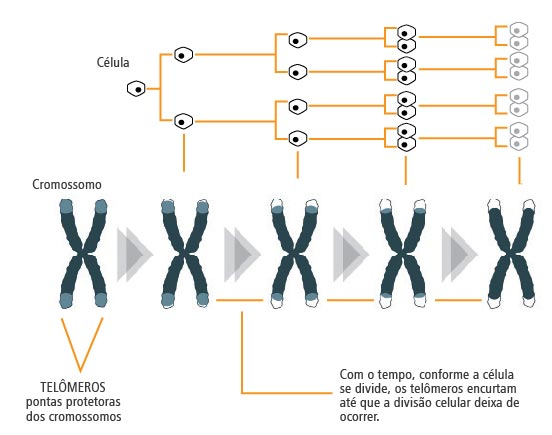
\includegraphics[width=0.7\textwidth]{Imagens/telomeros.jpg}
        }%
        \caption{Telômero}
        \label{fig:telomero}
    \end{figure}

    A principal função dos telômeros é proteger o DNA cromossômico durante a replicação e divisão celular. Como o DNA é replicado de maneira semi-descontínua e apenas em uma direção, as enzimas responsáveis pela replicação têm dificuldade em replicar completamente as extremidades dos cromossomos. Isso resultaria na perda de material genético a cada ciclo de replicação, comprometendo a informação genética e levando a danos nos genes essenciais.

    Os telômeros atuam como "capas" protetoras, evitando a perda de material genético nas extremidades cromossômicas. Eles têm uma estrutura especializada que permite que sejam reconhecidos e preservados pelas enzimas de replicação. Dessa forma, os telômeros impedem o encurtamento excessivo dos cromossomos ao longo do tempo e evitam que as extremidades cromossômicas sejam confundidas com danos ou quebras, que poderiam levar a rearranjos cromossômicos indesejados.

    Além de sua função protetora, os telômeros também estão envolvidos no controle do envelhecimento celular e no processo de senescência. À medida que as células se dividem repetidamente, os telômeros gradualmente encurtam até que a célula se torne senescente. O número de divisões que uma célula normal pode sofrer antes da senescência é conhecido como limite de Hayflick.

    A telomerase é uma enzima responsável por adicionar sequências de DNA repetitivas aos telômeros, compensando o encurtamento que ocorre naturalmente durante a replicação do DNA, ou seja, a telomerase permite que as células regenerem os telômeros. Isso ajuda a manter a estabilidade dos cromossomos e a capacidade das células se dividirem sem comprometer seu material genético.

    Nas células normais do nosso corpo, a expressão da telomerase é normalmente inativada ou muito baixa. Isso significa que, à medida que essas células se dividem repetidamente, seus telômeros encurtam progressivamente, limitando o número de vezes que elas podem se replicar. Eventualmente, os telômeros ficam muito curtos e as células entram em senescência ou morrem.

    As células-tronco imortais, como as células-tronco embrionárias, e as células germinativas, como os espermatozoides e óvulos, possuem uma alta expressão de telomerase. Isso lhes confere a capacidade de se autorrenovarem continuamente e de formar diferentes tipos de células especializadas ao longo do tempo, sem o encurtamento progressivo dos telômeros. Por outro lado, As células cancerígenas, devido às suas características anormais e capacidade de crescimento descontrolado, frequentemente reativam a expressão da telomerase. Isso permite que elas mantenham seus telômeros e continuem se dividindo indefinidamente, contribuindo para sua imortalidade celular e capacidade de formar tumores. Portanto, As células cancerígenas precisam expressar telomerase ou atividade semelhante à telomerase para manter sua capacidade de proliferar.

    








   


     
    
    



\bibliography{ref.bib}
\end{document}